%%%%%%%%%%%%%%%%%%%%%%%%%%%%%%%%%%%%%%%%%%%%%%%%%%%%%%%%%%%%%%%%%%%%%%%%%%%%%%%%
%2345678901234567890123456789012345678901234567890123456789012345678901234567890
%        1         2         3         4         5         6         7         8


\documentclass[conference]{IEEEtran}
\usepackage{cite}
\usepackage{amsmath,amssymb,amsfonts}
\usepackage{algorithmic}
\usepackage{graphicx}
\usepackage{textcomp}
\usepackage[justification=center]{caption}
\usepackage{xcolor}
\def\BibTeX{{\rm B\kern-.05em{\sc i\kern-.025em b}\kern-.08em
    T\kern-.1667em\lower.7ex\hbox{E}\kern-.125emX}}

\usepackage{eso-pic}
\usepackage{fancyhdr}
\usepackage{kantlipsum}

\fancyhf{}
\fancyfoot[L]{SCEES}    %%% change C to L or R as needed
\renewcommand{\headrulewidth}{0pt}
\renewcommand{\footrulewidth}{0pt}
\fancyhf{}

\fancyfoot[L]{SCEES}    %%% change C to L or R as needed
\renewcommand{\headrulewidth}{0pt}
\renewcommand{\footrulewidth}{0pt}

\fancypagestyle{plain}{
  \fancyhf{}
%  \fancyhead[L]{Conference on \LaTeX}     %% C or L or R.
  \fancyfoot[L]{This is a notice}%                        %% C or L or R.
  \renewcommand{\footrulewidth}{0pt} 
  \renewcommand{\headrulewidth}{0pt}
}



\AddToShipoutPictureBG*{%
  \AtPageLowerLeft{%
    \setlength\unitlength{1in}%
    \hspace*{\dimexpr0.225\paperwidth\relax}%%  change \dimexpr0.5\paperwidth\relax appropriately
    \makebox(0,1)[L]{978-1-7281-8876-8/21/\$31.00 \copyright2021 IEEE}%
}}   

\title{Pneumonia Detection from Chest X-ray using Transfer Learning}

%\author{ \parbox{3 in}{\centering Huibert Kwakernaak*
%         \thanks{*Use the $\backslash$thanks command to put information here}\\
%         Faculty of Electrical Engineering, Mathematics and Computer Science\\
%         University of Twente\\
%         7500 AE Enschede, The Netherlands\\
%         {\tt\small h.kwakernaak@autsubmit.com}}
%         \hspace*{ 0.5 in}
%         \parbox{3 in}{ \centering Pradeep Misra**
%         \thanks{**The footnote marks may be inserted manually}\\
%        Department of Electrical Engineering \\
%         Wright State University\\
%         Dayton, OH 45435, USA\\
%         {\tt\small pmisra@cs.wright.edu}}
%}

% author names and affiliations
% use a multiple column layout for up to three different
% affiliations
\author{
\IEEEauthorblockN{ Sharvari Kalgutkar , Vansh Jain , Gokul Nair , Kaustubh Venkatesh , Kshitij Parab , Amol Deshpande , Dayanand\\ Ambawade}
\IEEEauthorblockA{Department of Electronics and Telecommunications\\
Sardar Patel Institute of Technology\\
Mumbai-58, Maharashtra, India
}
}

\begin{document}

\maketitle
\thispagestyle{empty}
\pagestyle{empty}


%%%%%%%%%%%%%%%%%%%%%%%%%%%%%%%%%%%%%%%%%%%%%%%%%%%%%%%%%%%%%%%%%%%%%%%%%%%%%%%%
\begin{abstract}

The use of computing technology to aid modern medicine advancement has revolutionised healthcare. Quick and accurate diagnostic tools help professionals start the necessary treatment as soon as possible, saving millions of lives. Pneumonia, a symptom of Covid-19, is a life-threatening condition that affects the lungs and can be detected by analyzing X-ray scans of the chest. The study highlights Convolutional Neural Networks, develops and trains models such as VGG16, ResNet-50, and InceptionV3, to detect pneumonia with improved testing accuracies of 94 \%, 93.9 \%, and 93.5 \%, respectively. The work discusses and compares the implementation and performance of these models.


Keywords:  Pneumonia detection, CNN, ResNet, InceptionV3, VGG16, X-Rays, Deep Learning, Transfer Learning.

\end{abstract}


%%%%%%%%%%%%%%%%%%%%%%%%%%%%%%%%%%%%%%%%%%%%%%%%%%%%%%%%%%%%%%%%%%%%%%%%%%%%%%%%
\section{Introduction}

Pneumonia is an infection that develops inflammation in one or both lungs due to viruses, bacteria, fungi, or other germs. Primary infection happens when a person breathes in the air carrying germs, the airbags fill with pus and other liquids. There are two types of Pneumonia: bacterial and viral. Bacterial pneumonia causes more acute symptoms than viral Pneumonia. It is a common condition all over the world whose critical cause includes a high degree of pollution.

Acute respiratory infections, mainly caused by pollutants, sub-par hygiene levels, and bacterial infections, account for nearly 70 \% of India’s communicable diseases in 2018. In its evaluation, UNICEF placed India in the second position concerning the number of pneumonia deaths in the country [1].

According to the World Health Organization (WHO), the most common symptom of severe COVID-19 is pneumonia. Many mild cases of COVID-19 are diagnosed with mild pneumonia.[2]


The following processes can diagnose pneumonia: chest X-rays, Computerised Tomography (CT) of the lungs, chest ultrasound, lung needle biopsy, and magnetic resonance imaging of the chest. Chest X-rays are currently one of the best tools for diagnosing pneumonia. X-ray imaging is preferable over CT imaging since CT imagery typically takes much longer than X-ray imagery. In many underdeveloped areas, there may not be accessible, appropriate high-quality CT scanners available. By contrast, X-rays are the most common and cheaply accessible medical imaging procedures that contribute significantly to clinical care and epidemiological studies [3].



\section{Related Work}


Convolutional Neural Network (CNN) models are widely used to detect different kinds of pneumonia infections accurately. Cohen et al. study a model based on DenseNet-121 and has an accuracy of 92.8 \% and recall of 93.2 \% [4]. Ayan et al. use deep learning methods to create a model having an accuracy of 84.5 \% and recall of 89.1 \% [5]. In his study, [3] discusses using weighted classification models and has been able to achieve an AUC score of 99.76 \%. Findings from [6], [7], [8], [9], and [10] have accuracies ranging from 82-95 \%. They advocate the use of models such as Inception [6], ResNet [7], VGG [8], AlexNet [9],  DenseNet [10]. These methods use pre-trained models. The models achieve high accuracy values by feature extraction, and compensate for abnormalities in the real world. These models  do not always work well as mentioned [11] . Authors of [12] utilize a combination of CNN and classification algorithms to implement the DenseNet model.

The work's main contribution is the addition of a customized set of layers at the end of each transfer learning model. Addition of layers reduces overfitting. It increases the generalization of the models created.

The organization of the paper is as follows. Section III defines the significant concepts of Transfer learning with subsections explaining the models used. Section IV gives information about the architecture of the hybrid model developed. Section V talks about the methodology of implementation of the models used. Section VI takes us through the study’s outcome and the parameters used for performance evaluation, and its significance to the study’s result. Section VII concludes the study and summarizes the importance of finding a solution to pneumonia using artificial intelligence.



\section{Transfer Learning}

Transfer Learning is not a new concept in the machine learning world. It is the concept of reusing models developed for a task as a starting point for a second model. Transfer learning is an approach in deep learning which utilizes pre-trained models as the building blocks for a newer application. It uses only part of the pre-existing model saving the user vast computing power, time, and resources. These resources are mostly used for image classification problems which require more power and time to train layers.

In deep learning applications with a large and challenging image classification task, it is common to use ImageNet, a vast database of over 14 million images [13].


\begin{figure}
\centering
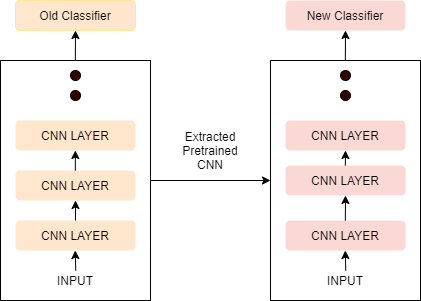
\includegraphics[width=6cm]{2.png}
\caption{ Representation of Transfer Learning}
\label{fig:cenario}
\end{figure}

Fig.1 explains the working of transfer learning in a block diagram. The new classifier extracts old pre-trained model layers and weights to train hence reducing computational complexity and saving time. The study uses three deep learning networks, namely, InceptionV3, VGG16, and Resnet 50 with an optimizer, namely Adam Optimizer.

\subsection{\centering{ Inception Model}}

Inception is a deep learning convolutional neural network developed by Google in 2015. Each layer is a combination of all the filters (1x1, 3x3, 5x5, and max-pooling). The results from these filters concatenate into a single vector. This single vector forms the input for the next layer. The InceptionV3 is a 48 layers deep neural network.

\subsection{\centering{ ResNet-50 Model}}
In ResNet-50, there is a  single Convolutional layer and Max Pooling. Four similar layers with varying filter sizes follow the above layers (using 3 x 3 convolution operations). The model bypasses or skips the layer in-between two successive convolutions. These skipped connections are known as ‘identity shortcut connections.’ These connections use residual blocks for carrying out the residual mapping that applies to all layers.

\subsection{\centering{ VGG16 Model}}
VGG16 is a convolutional neural network-based model developed in 2015. VGG16 improves the ALex Net model. VGG16 is  a  combination of convolution, max pooling, fully connected layers with an activation set to Relu, and an output layer. VGG16 has 16 layers. A remarkable property  of VGG16 is that max-pooling always performs over a 2x2 pixel window with a stride of 2. The filter size is 3x3.


\subsection{\centering{ Adam Optimizer}}

Adam Optimizer is a combination of Adaptive Gradient Algorithm and Root Mean Square Propagation. The algorithm’s learning rate parameters depend on the mean and the average of the second moments of the gradients (the uncentered variance). It works by calculating the exponential moving average of both the gradient and the squared gradient. The above parameters control the decay rates of these exponentially moving averages.  Adam optimizer decreases the training time, thus giving efficient results [14].





\section{Architecture using Transfer Learning}

Fig.2 shows the detailed architecture of each hybrid model. The pre-trained layers follow the input layer, followed by weights of InceptionV3, VGG16, and ResNet 50 models. The '?' in the architecture represents the number of images. A set of customized layers of flatten, dense, dropout, and global average are added to these pre-trained layers to enhance the pre-trained transfer learning models’ performance. The number of neurons in these customized layers gradually decreases to form a funnel. Funneling reduces the probability of the model overfitting the dataset.

\begin{figure}
\centering
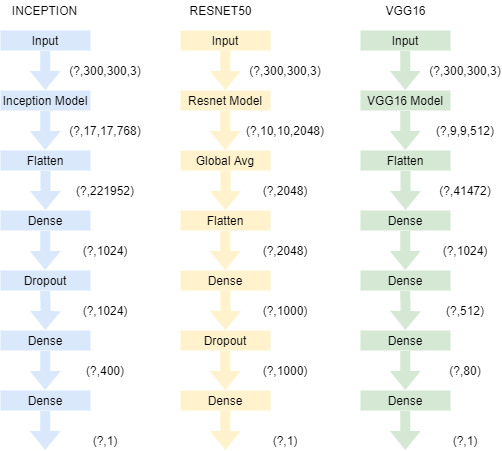
\includegraphics[width=9cm,height=7cm]{1.png}
\caption{a) InceptionV3 Model b) ResNet-50 Model c) VGG16 Model}
\label{fig:cenario}
\end{figure}

\section{Implementation}
This section contains an overview of the setup, data required, and the preprocessing to actively perform the study.

\subsection{\centering{ Experimental Dataset}}
The dataset used for the study is the Labeled Optical Coherence Tomography (OCT) and Chest X-ray Images for Classification Mendeley data set. It divides the data into three sections (train data, test data, validation). The data set contains 5,863 X-ray images (JPEGs) in two groups, namely pneumonia and normal.[15]

\begin{figure}
\centering
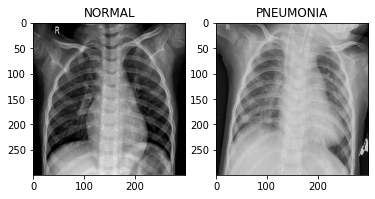
\includegraphics[width=8cm]{index.png}
\caption{Normal chest X-ray and Pneumonia positive chest X-ray }
\label{fig:cenario}
\end{figure}

In Fig.3, the second X-ray shows an area of lung inflammation, indicating a positive case for pneumonia. However, the first picture shows a standard chest X-Ray. The typical chest X-ray (left) shows areas without opacification of the lungs in the image. Bacterial pneumonia (right) exhibits consolidation of lobes of the lungs that infers an alveolar spread of infection, mainly because of the bacterium [16].


\subsection{\centering{ Experimental Setup}}
The study uses Google Colaboratory (based on Python) for data pre-processing, augmentation, model training, and testing with Tesla P100-PCIe-16GB GPU, disk space of 68.04 GB, RAM of 12.72 GB on a Standard PC. The necessary libraries used in this work are Keras, Tensorflow, NumPy, Matplotlib, Seaborn and Scikit-learn libraries.

\subsection{\centering{ Data Preprocessing and Augmentation}}
Models are generalised by providing a large amount of data. Training on a larger dataset achieves more significant efficiency. The dataset's size can be increased using data augmentation techniques. Data augmentation  provides more images for training the model. For the dataset preprocessing, all the images are converted into an array of size (300,300,3). The pixel values are rescaled  between 0 and 1. When reduced below (300,300,3), the image size resulted in a low-quality image, and the model’s performance is affected.
Data augmentation with the following parameters increases the size and the diversity of the dataset:-
Rotation range = 10 , Zoom range = 0.2, Shear Range=0, Horizontal Flip = False, Width Shift Range = 0.2, Height Shift Range = 0.2 .


\subsection{\centering{ Fine-Tuning  Model Parameters}}
The dataset contains 25\% Normal chest X-ray images and 75\% pneumonia chest X-ray images. Class weights computation is necessary because of imbalance in the dataset. Training the model utilizes these class weights. All three models have the number of epochs set to 25. The batch size decides the number of images trained at a given time. It improves accuracy and reduces the training time of the model. By convention, the study sets the batch size to the power of 2 (e.g., 16, 32, 64, etc.). A lower value of batch size causes the model to never converge at the global minima, and a higher value of batch size causes poor generalization of the model. Therefore, the batch size is set to 32. All the layers are trainable. The work sets compilation loss to  binary cross-entropy and the optimizer as Adam. The learning rate is  10$^{-4}$. 

\section{Results}
The results section presents the evaluation metrics to test the above trained models’ efficiency. The models use the following metrics to evaluate their performance: Binary Accuracy, Area Under Curve (AUC), Recall with a threshold of 0.5, Precision with a threshold of 0.5, and Confusion Matrix. Binary classification accuracy is :


\begin{equation}
   Accuracy=\frac{TP +TN}{TP +TN + FP +FN}
\end{equation}

where,
\newline
TP = True Positive , TN = True Negative \newline
FP = False Positive , FN = False Negative  
\newline
\par
Binary accuracy closer to 1 implies the model successfully classifies pneumonia chest X-ray. However, accuracy cannot be considered as the only deciding metric as the dataset is imbalanced. Receiver Operating Characteristic curve (ROC), is a True Positive rate plot versus a False Positive rate. AUC is a measure of the 2-dimensional area under the ROC curve. AUC has a range of 0 to 1. A model whose prediction is 100 percent wrong has an AUC of 0, while a model whose predictions are 100 percent correct has an AUC of 1. Therefore, concluding that the Area Under Curve (AUC) is a better metric. 

Since the work aims to detect pneumonia based on chest X-ray, it is vital to reduce the model’s false-negative rate. It is vital for such a model to accurately detect which people are suffering from pneumonia, thus ensuring timely treatment. Recall's formula is:

\begin{equation}
   Recall=\frac{TP}{TP + FN}
\end{equation}


\par
Improving the model's recall decreases the false-negative rate. Thus for detecting pneumonia based on chest X-ray recall value closer to 1 ensures better performance. The precision of a model is:

\begin{equation}
   Precision=\frac{TP}{TP + FP}
\end{equation}


Precision closer to 1 implies better performance than closer to 0.
\newline
\par
Confusion Matrix is a tabular representation that evaluates the performance of a classification model. It compares the predicted and actual values for a model.

\begin{table}[]
\centering
\caption{Confusion Matrix}
\begin{tabular}{|c|c|c|}
\hline
                                                             & \begin{tabular}[c]{@{}c@{}}\rule{0pt}{10pt}PREDICTED\\ (Normal)\end{tabular} & \begin{tabular}[c]{@{}c@{}}\rule{0pt}{10pt}PREDICTED\\ (Pneumonia)\end{tabular} \\ \hline
\begin{tabular}[c]{@{}c@{}}\rule{0pt}{10pt}ACTUAL\\ (Normal)\end{tabular}    & TN                                                           & FP                                                              \\ \hline
\begin{tabular}[c]{@{}c@{}}\rule{0pt}{10pt}ACTUAL\\ (Pnuemonia)\end{tabular} & FN                                                           & TP                                                              \\ \hline
\end{tabular}
\end{table}

Table I represents a basic confusion matrix. The columns of the matrix represent the predicted values, while the row shows the actual values. The sum of a row is equal to the number of cases of a particular class, and the sum of all cells is equal to the total test cases. For a particular chest X-ray, if the model predicts pneumonia chest X-ray correctly, it is True Positive. If the model predicts Normal chest X-ray correctly, it is  True Negative. If the original image is of Normal chest X-ray and the predicted label is pneumonia chest X-ray , it is False Positive. If the original image is of pneumonia chest X-ray and the predicted label is Normal chest X-ray, it is False Negative. 

Table II, III, IV  summarizes accuracy, precision, recall, AUC, the loss for train-set, validation-set, and test-set, respectively. These results are obtained by training the three models for 25 epochs. 

\begin{table}[]
\caption{Training  performance}
\resizebox{245pt}{!}{%
\begin{tabular}{|c|c|c|c|c|c|}
\hline
\multicolumn{6}{|c|}{\rule{0pt}{20pt}TRAINING PERFORMANCE} \\ \hline
\rule{0pt}{20pt}Model         & Loss    & Accuracy  & AUC     & Recall & Precision \\ \hline
\rule{0pt}{20pt}VGG16        & 0.0317  & 0.9884    & 0.9987  & 0.9873 & 0.9971    \\ \hline
\rule{0pt}{20pt}InceptionV3  & 0.0187  & 0.9967    & 0.9996  & 0.9907 & 0.9979    \\ \hline
\rule{0pt}{20pt}ResNet 50     & 0.0116  & 0.9952    & 0.9999  & 0.9946 & 0.9990    \\ \hline
\end{tabular}%
}
\end{table}

\begin{table}[]
\caption{Validation  performance}
\resizebox{245pt}{!}{%
\begin{tabular}{|c|c|c|c|c|c|}
\hline
\multicolumn{6}{|c|}{\rule{0pt}{20pt}VALIDATION PERFORMANCE} \\ \hline
\rule{0pt}{20pt}Model         & Loss     & Accuracy   & AUC   & Recall  & Precision  \\ \hline
\rule{0pt}{20pt}VGG16        & 0.0070   & 1.00       & 1.00  & 1.00    & 1.00       \\ \hline
\rule{0pt}{20pt}InceptionV3   & 0.2367   & 0.9375     & 1.00  & 0.875   & 1.00       \\ \hline
\rule{0pt}{20pt}ResNet 50     & 0.1121   & 0.9375     & 1.00  & 1.00    & 0.8889     \\ \hline
\end{tabular}%
}
\end{table}

\begin{table}[]
\caption{Test  performance}
\resizebox{245pt}{!}{%
\begin{tabular}{|c|c|c|c|c|c|}
\hline
\multicolumn{6}{|c|}{\rule{0pt}{20pt}TEST PERFORMANCE} \\ \hline
\rule{0pt}{20pt}Model        & Loss   & Accuracy & AUC    & Recall & Precision \\ \hline
\rule{0pt}{20pt}VGG16       & 0.2063 & 0.9407   & 0.9796 & 0.9667 & 0.9401    \\ \hline
\rule{0pt}{20pt}InceptionV3 & 0.3994 & 0.9359   & 0.9651 & 0.9513 & 0.9464    \\ \hline
\rule{0pt}{20pt}ResNet 50    & 0.2755 & 0.9391   & 0.9694 & 0.9897 & 0.9190    \\ \hline
\end{tabular}%
}
\end{table}

Table IV summarizes the test performance for different models. VGG16  attains the highest test accuracy of 0.9407 and minimum testing loss of 0.2063. ResNet-50 closely follows VGG16 with an accuracy of 0.9391 and loss of 0.2755. InceptionV3  has the lowest test accuracy of 0.9359 and highest testing loss of 0.3994. Among the three models, VGG16 attains the highest AUC of 0.9796, followed by ResNet-50 and InceptionV3. ResNet-50 has the highest recall of 0.9897, followed by VGG16 with a recall of 0.9667. InceptionV3 attains the highest precision of 0.9464.

Fig. 5, 6, 7, 8 show the curves for loss, accuracy, AUC, recall and precision of training and validation sets obtained while training the models for 25 epochs.

\begin{figure}
\centering
 \vspace{\floatsep}
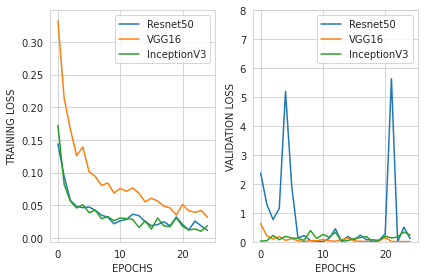
\includegraphics[width=8cm]{loss.png}
\caption{Training and Validation set Loss}
\label{fig:cenario}
\end{figure}
\begin{figure}
\centering
 \vspace{\floatsep}
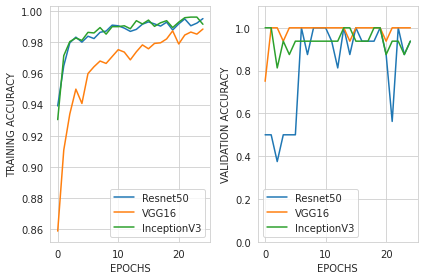
\includegraphics[width=8cm]{accuracy.png}
\caption{Training and Validation set Accuracy}
\label{fig:cenario}
\end{figure}
\begin{figure}
\centering
 \vspace{\floatsep}
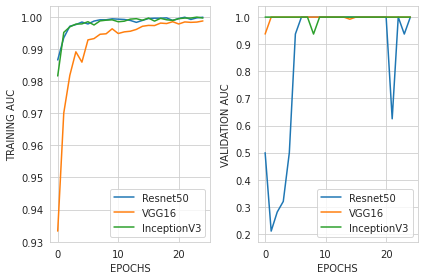
\includegraphics[width=8cm]{auc.png}
\caption{Training and Validation set AUC}
\label{fig:cenario}
\end{figure}
\begin{figure}
\centering
 \vspace{\floatsep}
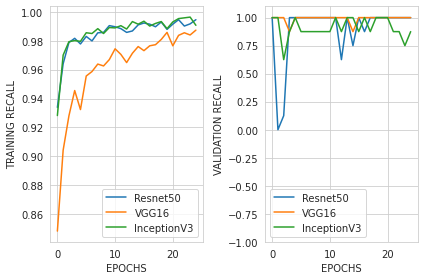
\includegraphics[width=8cm]{recall.png}
\caption{Training and Validation set Recall}
\label{fig:cenario}
\end{figure}
\begin{figure}
\centering
 \vspace{\floatsep}
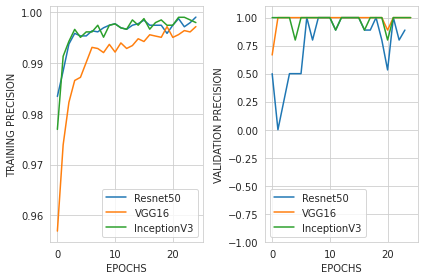
\includegraphics[width=8cm]{precision.png}
\caption{Training and Validation set Precision}
\label{fig:cenario}
\end{figure}
 
Fig. 9 depicts the confusion matrix for InceptionV3. The Inception model correctly predicts 213 out of  234 normal chest X-rays and misclassifies 21 normal chest X-rays as pneumonia. InceptionV3 correctly predicts 371 of 390 pneumonia chest X-rays. It misclassifies 19 pneumonia X-rays as a normal chest X-ray.


\begin{figure}
\centering
 \vspace{\floatsep}
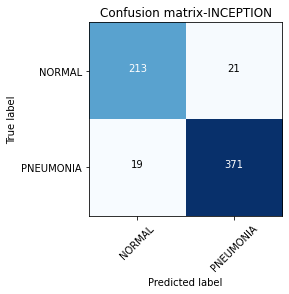
\includegraphics[width=6cm]{CMINCEP.png}
\caption{Confusion matrix  of InceptionV3  based model}
\label{fig:cenario}
\end{figure}

Fig. 10 is a plot of the confusion matrix for ResNet-50. It correctly predicts 200 out of  234 normal chest X-rays. ResNet-50 misclassifies  34  normal chest X-rays as pneumonia. The Restnet-50 model accurately predicts 386 out of 390 pneumonia chest X-rays. It  misclassifies  4 pneumonia chest X-ray as normal.

\begin{figure}
\centering
  \vspace{\floatsep}
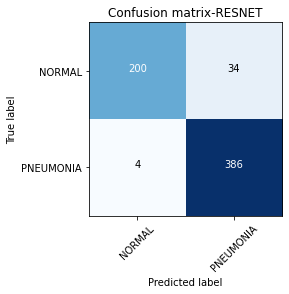
\includegraphics[width=6cm]{CMRES.png}
\caption{Confusion matrix  of ResNet 50 based model}
\label{fig:cenario}
\end{figure}
\begin{figure}
\centering
 \vspace{\floatsep}
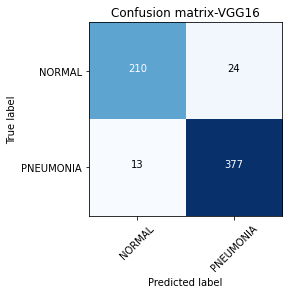
\includegraphics[width=6cm]{CMVGG.png}
\caption{Confusion matrix  of VGG16 based model}
\label{fig:cenario}
\end{figure}

Fig. 11 is a plot of the confusion matrix for VGG16. The model correctly predicts 210 out of  234 normal chest X-rays. VGG16 misclassifies  24 regular chest X-rays as pneumonia. The VGG16 model rightly classifies  377 out of 390 pneumonia chest X-rays. It misclassifies 13 pneumonia chest X-rays as normal.


The performance of InceptionV3 in comparison to the other two models is lacking in terms of its accuracy, loss, recall, precision and AUC. VGG16 has the maximum accuracy, AUC, and minimum loss. It has a lower recall compared to ResNet-50. ResNet 50 has accuracy, precision, AUC and loss comparable to that of VGG16. The Recall of ResNet-50 is high, ensuring a low false-negative rate, which is important for pneumonia prediction using chest X-ray. Thus considering the above metrics ResNet-50 exhibits the best overall performance.


\section{Conclusion}
Pneumonia is a deadly disease that affects the lungs. Early diagnosis helps doctors provide care without any adverse complications. The inspiration for the paper is the global nature of the problem. Pneumonia causes more than 2.7 million fatalities. Thus, an accurate, rapid, and generalized diagnosis solution is of utmost importance.

Moreover, many medical facilities worldwide are unable to examine X-rays accurately. The study aims at solving these problems using concepts of Transfer Learning and Convolutional Neural Networks.

This study focuses on CNN models like InceptionV3, ResNet-50, and VGG16 based on Transfer Learning specifically for pneumonia detection. The work achieves increased accuracy values by 5-7 \% after adding a set of customized neural layers. The addition of the customized layers and data augmentation avoids overfitting of complex transfer learning models on limited data. 

The study builds and compares the models based on the No Free Lunch Theorem. Plotting and analyzing the metadata generated during the training of the models helped in determining the best model.

The work compares the model performances using metrics like precision, recall, AUC, accuracy, loss, and confusion matrix which helps evaluate the three models’ robustness on training, validation, and test datasets. All models achieve training accuracies above 98 \% and an AUC value of 1. 

VGG16 achieves the highest validation accuracy and testing accuracy of 94.07 \% and AUC  of 97.96 \%. The recall of VGG16 is less compared to ResNet-50. It is essential to reduce false negatives while increasing the accuracy and AUC of the models. 

ResNet-50 shows better performance across all parameters. ResNet-50 attains a maximum recall of 98.97 \%, testing accuracy of  93.91 \%, and AUC of 96.94 \%.
  
After averaging the performance parameters (precision, recall, loss, accuracy, and AUC), this work concludes that the ResNet-50 model performs the best.

Future studies can consider model weights corresponding to different algorithms, making the process more efficient and can increase the accuracy and recall of the models. The models can also incorporate patients’ historical data to give a more detailed and conclusive report of the X-ray diagnosis.




\addtolength{\textheight}{-12cm}   % This command serves to balance the column lengths
                                  % on the last page of the document manually. It shortens
                                  % the textheight of the last page by a suitable amount.
                                  % This command does not take effect until the next page
                                  % so it should come on the page before the last. Make
                                  % sure that you do not shorten the textheight too much.

%%%%%%%%%%%%%%%%%%%%%%%%%%%%%%%%%%%%%%%%%%%%%%%%%%%%%%%%%%%%%%%%%%%%%%%%%%%%%%%%


\bibliographystyle{IEEEtran}  
\bibliography{IEEEexample}


[1] Sneha Moradni, “Biggest Killer Infection in India,      Pollution Worsening Crisis, Says Report”, News 18  India,      12 November 2017.
\newline

[2] Zawn Villines, “ Pneumonia and COVID-19: Relationship, risks, and more”, Medical News Today, 15 April 2020. 
\newline

[3] Hashmi, Mohammad Farukh et al. “Efficient Pneumonia Detection in Chest X Ray Images Using Deep Transfer Learning.” Diagnostics (Basel, Switzerland) vol. 10,6 417. 19 Jun. 2020, doi:10.3390/diagnostics10060417.
\newline

[4] Cohen J.P., Bertin P., Frappier V. Chester: A Web Delivered Locally Computed Chest X-Ray Disease Prediction System. arXiv. 20191901.11210.
\newline

[5]  Ayan E., Ünver H.M. Diagnosis of Pneumonia from Chest X-Ray Images Using Deep Learning; Proceedings of the 2019 Scientific Meeting on Electrical-Electronics \& Biomedical Engineering and Computer Science (EBBT); Istanbul, Turkey. 2–26 April 2019; pp. 1–5.
\newline

[6] C. Szegedy et al., "Going deeper with convolutions," 2015 IEEE Conference on Computer Vision and Pattern Recognition (CVPR), Boston, MA, 2015, pp. 1-9, doi: 10.1109/CVPR.2015.7298594.
\newline

[7]  K. He, X. Zhang, S. Ren and J. Sun, "Deep Residual Learning for Image Recognition," 2016 IEEE Conference on Computer Vision and Pattern Recognition (CVPR), Las Vegas, NV, 2016, pp. 770-778, doi: 10.1109/CVPR.2016.90.
\newline

[8] S. Liu and W. Deng, "Very deep convolutional neural network based image classification using small training sample size," 2015 3rd IAPR Asian Conference on Pattern Recognition (ACPR), Kuala Lumpur, 2015, pp. 730-734, doi: 10.1109/ACPR.2015.7486599.
\newline

[9] Krizhevsky, Alex; Sutskever, Ilya; Hinton, Geoffrey E. (2017-05-24). "ImageNet classification with deep convolutional neural networks" (PDF). Communications of the ACM. 60 (6): 84–90. doi:10.1145/3065386. ISSN 0001-0782.
\newline

[10]  Gao Huang, Zhuang Liu, Laurens van der Maaten, Kilian Q. Weinberger “Densely Connected Convolutional Networks”   arXiv:1608.06993 [cs.CV]   28 Jan 2018.
\newline

[11] Pranav Rajpurkar, Jeremy Irvin, Kaylie Zhu, Brandon Yang, Hershel Mehta, Tony Duan, Daisy Ding, Aarti Bagul, Curtis Langlotz, Katie Shpanskaya, Matthew P. Lungren, Andrew Y. Ng et al. “CheXNet: Radiologist-Level Pneumonia Detection on Chest X-Rays with Deep Learning” arXiv:1711.05225v3 [cs.CV] 25 Dec 2017.
\newline

[12]  D. Varshni, K. Thakral, L. Agarwal, R. Nijhawan and A. Mittal, "Pneumonia Detection Using CNN based Feature Extraction," 2019 IEEE International Conference on Electrical, Computer and Communication Technologies (ICECCT), Coimbatore, India, 2019, pp. 1-7, doi: 10.1109/ICECCT.2019.8869364.
\newline

[13] Wikipedia contributors. "ImageNet." Wikipedia, The Free Encyclopedia. Wikipedia, The Free Encyclopedia, 1 Dec. 2020. Web. 27 Dec. 2020.
\newline

[14]  Diederik P. Kingma, Jimmy Ba “Adam: A Method for Stochastic Optimization” arXiv:1412.6980 [cs.LG] 30 Jan 2017.
\newline

[15] Kermany, Daniel; Zhang, Kang; Goldbaum, Michael (2018), “Labeled Optical Coherence Tomography (OCT) and Chest X-Ray Images for Classification”, Mendeley Data, V2, doi: 10.17632/rscbjbr9sj.2.
\newline

[16] Mooney, P.(2018, March 24). Chest X-Ray Images (Pneumonia). Retrieved December 27, 2020, from https://www.kaggle.com/paultimothymooney/chest-xray-pneumonia.
\newline
\end{document}
